\documentclass{article}
\usepackage[a4paper, paperwidth=25cm, paperheight=25.5cm, left=1.5cm, right=1.5cm, top=1cm, bottom=2cm]{geometry}
\usepackage{tikz,tcolorbox}
\usepackage{amsmath}
\usepackage[table,xcdraw]{xcolor}
\usepackage{listings}
\usepackage{array,multirow} % For customizing tables
\usepackage{booktabs} % For better horizontal lines
\usepackage{makecell}
\setlength{\parindent}{0pt}

\usepackage{algorithm}
\usepackage{algpseudocode}

\tcbuselibrary{skins, breakable, theorems}

\definecolor{myblue}{HTML}{10C2C4}

\newtcolorbox{prettyBox}[2]{
  enhanced,
  colback=white!90!#2,   % Background color based on the second parameter (color)
  colframe=#2!60!black,  % Frame color based on the second parameter (color)
  coltitle=white,        % Title color (white)
  fonttitle=\bfseries\Large,
  title=#1,              % Title from the first parameter
  boxrule=1mm,
  arc=0.5mm,
  drop shadow=#2!35!gray, % Drop shadow color based on the second parameter (color)
}

\usepackage{listings}
% Define the style for C code
\lstdefinestyle{cstyle}{
    language=C,
    basicstyle=\ttfamily\small,
    keywordstyle=\color{blue}\bfseries,
    stringstyle=\color{red},
    commentstyle=\color{green!50!black}\itshape,
    numbers=left,
    numberstyle=\tiny\color{gray},
    stepnumber=1,
    breaklines=true,
    frame=tb,
    tabsize=4,
    showstringspaces=false,
    captionpos=b
}


\lstdefinestyle{pythonstyle2}{
    language=python,                    % Language set to Python
    basicstyle=\ttfamily\footnotesize,   % Change basic font size
    keywordstyle=\color{blue}\bfseries, % Different keyword style
    stringstyle=\color{red},         % Different string color
    commentstyle=\color{green!60!black}\itshape, % Adjust comment color
    numbers=left,                       % Line numbers on the left
    numberstyle=\tiny\color{gray},      % Smaller number font and color
    stepnumber=1,                       % Number each line
    frame=single,                       % Single frame around code
    tabsize=4,                          % Adjust tab size
    showstringspaces=false,             % Do not show spaces in strings
    captionpos=b,% Position of caption
    breaklines=true,
    inputencoding=utf8
}

\definecolor{redPlot}{HTML}{ED014A}

\algrenewcommand\algorithmicif{\textcolor{redPlot}{\textbf{if}}}
\algrenewcommand\algorithmicelse{\textcolor{redPlot}{\textbf{else}}}
\algrenewcommand\algorithmicprocedure{\textcolor{redPlot}{\textbf{procedure}}}

\algrenewcommand\algorithmicfunction{\textcolor{redPlot}{\textbf{function}}}
\algrenewcommand\algorithmicend{\textcolor{redPlot}{\textbf{end}}}
\algrenewcommand\algorithmicthen{\textcolor{redPlot}{\textbf{then}}}

\algrenewcommand\algorithmicdo{\textcolor{redPlot}{\textbf{do}}}
\algrenewcommand\algorithmicwhile{\textcolor{redPlot}{\textbf{while}}}

\algrenewcommand\algorithmicfor{\textcolor{redPlot}{\textbf{for}}}


\setlength{\arrayrulewidth}{0.8mm} % Set border thickness
\setlength{\tabcolsep}{12pt} % Set column margin

\renewcommand{\arraystretch}{1.5} % Increase row height for better vertical spacing
\begin{document}
\begin{center}
    \Huge{\textbf{\underline{Chapter 1: Introduction}}}
\end{center}

\vspace{0.35cm}


\section{Numerical Algorithm (Numerical Method)}
\begin{prettyBox}{Numerical Algorithm}{mygreen}
A Numerical Algorithm provides an approximate solution and is used to solve problems involving large amounts of data. The algorithm is based on a well-defined iterative sequence, starting with an initial solution that progressively converges toward the desired result with each iteration.

\[
\begin{cases}
    \hspace{0.1cm}(U_n) & \hspace{-0.1cm}n \geq 0 \\[0.15cm]
    \hspace{0.1cm}S_0 & \hspace{-0.3cm} \text{Initial Solution (Starting Point)}
\end{cases}
\]
\end{prettyBox}
\vspace{0.35cm}

\section{Convergence Speed (Order of Convergence)}
\begin{prettyBox}{Convergence Speed}{mygreen}
The number of iterations required to find the solution we are looking for:
\begin{itemize}
    \item Linear Order: 1 (slow)
    \item Quadratic Order: 2 (faster)
    \item \(>>\) 2 (very fast)
\end{itemize}
\end{prettyBox}

\vspace{0.35cm}

\section{Interpolation}
\begin{prettyBox}{Interpolation}{mygreen}
Estimates the value between two known points of a function allowing for a smoother representation of the function's behavior.
\end{prettyBox}

\vspace{0.35cm}

\section{Approximation}
\begin{prettyBox}{Approximation}{mygreen}
Approximates the formula of a function from a set of values, with the objective of finding a simpler function that represents the general trend of the data, even if it doesn't pass through every point exactly.
\end{prettyBox}

\vspace{0.35cm}

\section{Error}
\begin{prettyBox}{Error}{mygreen}
An error represents the difference between the actual solution and the computed result. It indicates how far we are from the true solution. There are two cases:
\begin{itemize}
    \item \textbf{Evaluation}: We know the exact solution, so we can directly calculate the error:
        \[   \boxed{E_r = |\overline{x} - x_{\text{app}}|} \]
    \item \textbf{Estimation}: We don't know the exact solution, so we only have an estimate of the error, based on the output of the algorithm:
        \[      \boxed{E_r = |\overline{x} - x_{\text{app}}| \leq \text{Algo}} \]
\end{itemize}

Where:
\begin{itemize}
    \item \(E_r\) : The error value.
    \item \(\overline{x}\) : The exact solution.
    \item \(x_{\text{app}}\) : The approximate solution.
    \item Algo : The error value found by the algorithm.
\end{itemize}
\end{prettyBox}

\vspace{0.35cm}

\section{Optimization}
\begin{prettyBox}{Optimization}{mygreen}
Optimization in numerical algorithms refers to two things:
\begin{itemize}
    \item \textbf{Error}: We aim to minimize the error in order to achieve the most accurate approximate solution.
    \item \textbf{Convergence Speed}: The higher the order of convergence, the less time the algorithm will take to converge to the solution we are looking for.
\end{itemize}
\end{prettyBox}

 
\newpage
\null
\vspace{0.15cm}

\begin{center}
    \Huge{\textbf{\underline{Chapter 1: State Space Search}}}
\end{center}

\setcounter{section}{0}

\vspace{0.35cm}


\section{State Space Search}
\begin{prettyBox}{Definition}{myblue}
State space search does not rely on prior experience. It involves solving a problem by exploring possible states and actions. The process includes:
\begin{enumerate}
    \item \textbf{Modeling the Problem:} Represent the problem using simple or complex data structures.
    \item \textbf{Defining the Search Space:}
        \begin{itemize}
            \item \textbf{Set of States:} Includes the initial state (\(S\)), the goal state (\(G\)), and all intermediate states.
            \item \textbf{Set of Legal Moves:} Represents the actions that allow transitions from one state to another.
        \end{itemize}
    \item \textbf{Defining Functions:}
        \begin{itemize}
            \item \textbf{Movegen(S: state):} Returns a set of states representing the results of all legal moves from the given state.
            \item \textbf{GoalTest(S: state):} Takes a state as input and returns a boolean value, verifying whether the given state is a goal state.
        \end{itemize}
\end{enumerate}
\end{prettyBox}

\vspace{0.35cm}

\begin{prettyBox}{Types of Problems}{myblue}
\begin{itemize}
    \item \textbf{Configuration Problems:} 
    The goal state is not explicitly defined but is identified by its properties. The concept of a path solution is irrelevant; only the goal state is retrieved.
    \item \textbf{Planning Problems:} 
    The goal state is explicitly defined, and the solution involves finding the path to reach the goal state.
\end{itemize}
\end{prettyBox}

\vspace{0.35cm}

\begin{prettyBox}{Note}{red}
Search-based agents are not highly efficient due to the issue of combinatorial explosion. As the search tree grows deeper, the number of nodes increases exponentially, resulting in an unmanageable number of possibilities to explore.
\end{prettyBox}

\vspace{0.35cm}

\begin{prettyBox}{Search Categories}{myblue}
\begin{itemize}
    \item \textbf{Uninformed Search:} Conducted without any guidance or additional data (blind search).
    \item \textbf{Informed Search:} Guided by additional information or heuristics.
\end{itemize}
\end{prettyBox}

\newpage
\subsection*{\underline{Example}}

\vspace{0.5cm}
\begin{prettyBox}{8-Puzzle Problem}{myblue}
The 8-puzzle problem consists of a \(3 \times 3\) matrix with integers from 1 to 8 placed randomly, along with an empty cell represented by \(X\). The goal is to rearrange the matrix to achieve the following configuration:
\end{prettyBox}

\vspace{0.65cm}
\begin{center}
    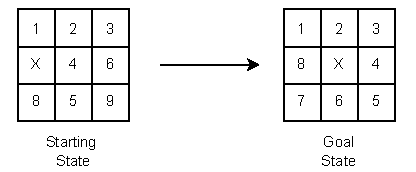
\includegraphics[width=0.6\textwidth]{Chapters/Example/Uninformed/ex1.drawio.pdf}
\end{center}

\vspace{0.45cm}

\begin{prettyBox}{Legal Moves}{myblue}
\begin{itemize}
    \item Slide Up
    \item Slide Down
    \item Slide Right
    \item Slide Left
\end{itemize}
\end{prettyBox}

\vspace{0.45cm}

\begin{prettyBox}{Representation}{myblue}
The matrix can be represented as a 2D array of integers, with the empty cell (\(X\)) optionally represented as \texttt{nil}.
\end{prettyBox}


\vspace{0.35cm}


\begin{prettyBox}{River Crossing Problem}{myblue}
This problem involves a man, a lion, a goat, a cabbage, a boat, and a river. Initially, all entities are on the left side of the river. The goal is to transport all of them to the right side without any entity being harmed:
\begin{itemize}
    \item If the lion and goat are left alone, the lion will kill the goat.
    \item If the goat and cabbage are left alone, the goat will eat the cabbage.
\end{itemize}
\end{prettyBox}


\vspace{0.5cm}
\begin{center}
    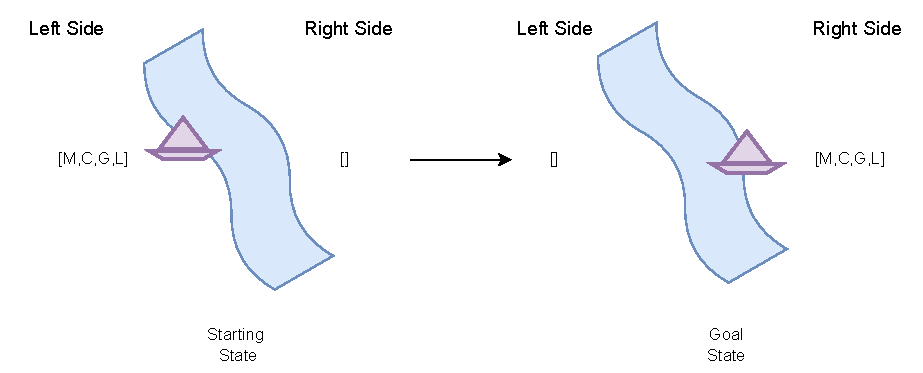
\includegraphics[width=0.8\textwidth]{Chapters/Example/Uninformed/ex2.1.drawio.pdf}
\end{center}

\vspace{0.5cm}
\begin{prettyBox}{Legal Moves}{myblue}
\begin{itemize}
    \item Man takes nothing to the right side.
    \item Man takes the cabbage.
    \item Man takes the lion.
    \item Man takes the goat.
\end{itemize}
\end{prettyBox}

\vspace{0.5cm}
\begin{prettyBox}{Representation}{myblue}
A list of structures, where each structure has the following fields:
\begin{itemize}
    \item \texttt{char name}: The name of the entity (\texttt{'M'} Man , \texttt{'C'} Cabbage, \texttt{'L'} Lion ,\texttt{'G'} Goat).
    \item \texttt{char position}: The position of the entity (\texttt{'L'} Left side, \texttt{'R'} Right side).
\end{itemize}

If any entity is harmed (eaten or killed), it is removed from the list, signifying its destruction.
\end{prettyBox}

\vspace{0.5cm}
\begin{center}
    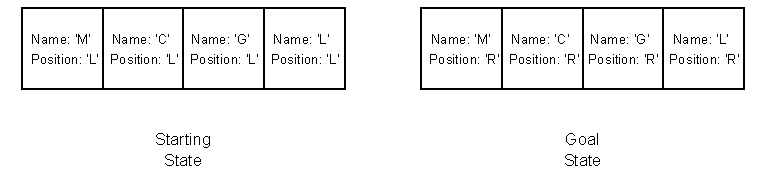
\includegraphics[width=0.8\textwidth]{Chapters/Example/Uninformed/ex2.2.drawio.pdf}
\end{center}

 
\newpage
\null
\begin{center}
    \Huge{\textbf{\underline{Chapter 1.1: Uninformed}}}
\end{center}

\setcounter{section}{0}

\vspace{0.35cm}
\section{Searching Algorithms}

\subsection{Simple Search 1}

\begin{algorithm}[ht]
\caption{SS1}
\begin{algorithmic}
\State Open \(\gets\) \{S\};
\vspace{0.1cm}
\While{ Open \(\neq\) nil}
\State N \(\gets\) Remove node from Open;

\vspace{0.07cm}
\If{(GoalTest(N))}
\State return N;
\Else
\State Open \(\gets\) Open \(\bigcup\) MoveGen(N);
\EndIf

\vspace{0.07cm}
\EndWhile

\vspace{0.1cm}
\State return nil;
\end{algorithmic}
\end{algorithm}

\vspace{0.35cm}
\begin{prettyBox}{Issues With SS1}{red}
It can infinitly loop because we aren't keeping track
of node we already seen to fix that we will use another list
to mark seen nodes
\end{prettyBox}

\vspace{0.75cm}
\subsection{Simple Search 2}

\begin{algorithm}[ht]
\caption{SS2}
\begin{algorithmic}
\State Open \(\gets\) \{S\};
\State Closed \(\gets\) \{\}; \Comment{Seen Node List}
\vspace{0.1cm}
\While{ Open \(\neq\) nil}
\State N \(\gets\) Remove node from Open;

\vspace{0.07cm}
\If{(GoalTest(N))}
\State return N;
\Else

\State Closed \(\gets\) Closed \(\bigcup\) \{N\};
\State Open \(\gets\) Open \(\bigcup\) ( MoveGen(N) \textbackslash\hspace{0.1cm}(Open \(\bigcup\) Closed)); \Comment{Append With No Duplicates}
\EndIf

\vspace{0.07cm}
\EndWhile

\vspace{0.1cm}
\State return nil;
\end{algorithmic}
\end{algorithm}


\begin{prettyBox}{Issues with SS2}{red}
Issue is the current algo only return the goal state and not the path,
this would be enough if we are in the context of configuration problem
but in case of planning problem we must have the path to fix that we will use
current parent node pair representation
\end{prettyBox}

\vspace{0.35cm}
\begin{center}
    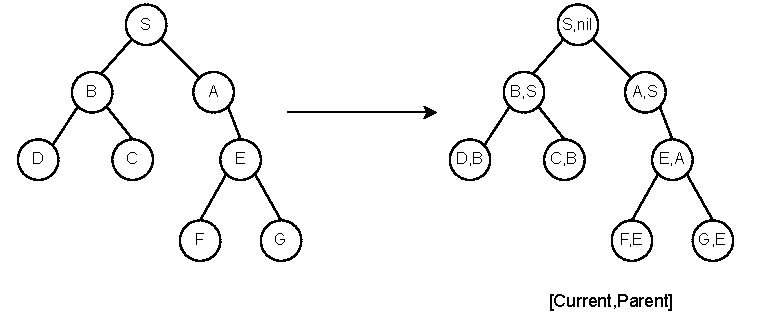
\includegraphics[height=0.3\textheight]{Chapters/Diagram/parent.drawio.pdf}
\end{center}



\vspace{0.5cm}
\subsection{Simple Search 3}

\begin{algorithm}[ht]
\caption{SS3}
\begin{algorithmic}
\State Open \(\gets\) \{\{S,nil\}\};
\State Closed \(\gets\) \{\};
\vspace{0.1cm}
\While{ Open \(\neq\) nil}
\State N \(\gets\) Remove node from Open;

\vspace{0.07cm}
\If{(GoalTest(N.current))}
\State return reconstructPath(N, Closed);
\Else

\State Closed \(\gets\) Closed \(\bigcup\) \{N\};
\State Open \(\gets\) Open \(\bigcup\) ( MoveGen(N) \textbackslash\hspace{0.1cm}(Open \(\bigcup\) Closed));
\EndIf

\vspace{0.07cm}
\EndWhile

\vspace{0.1cm}
\State return nil;
\end{algorithmic}
\end{algorithm}

\newpage
\null
\begin{algorithm}[ht]
\caption{reconstructPath}
\begin{algorithmic}
\Function{reconstructPath}{(I/N:(current,parent),Closed : List{(current,parent)}): List}
\State path \(\gets\) \{N.Current\};
\State N \(\gets\) find node in Closed where N.parent = Closed.current 
\vspace{0.1cm}
\While{ N.parent \(\neq\) nil}
\State path \(\gets\) path \(\bigcup\) \{N.Current\};
\State N \(\gets\) find node in Closed where N.parent = Closed.current 
\EndWhile
\vspace{0.1cm}
\State return reverse(Path);
\EndFunction
\end{algorithmic}
\end{algorithm}

\vspace{0.35cm}

\begin{prettyBox}{How To Choose N}{red}
We have two choices for selecting \( N \): either the head or the tail. The behavior of each choice differs as follows:
\begin{itemize}
    \item \textbf{Head:} If we choose the head, it is treated as a queue. In this case, we \textit{reappend} the state to the end of the structure, effectively following a breadth-first search approach.
    \item \textbf{Tail:} If we choose the tail, it is treated as a stack. We simply \textit{append} the state to the end of the structure, following a depth-first search approach.
\end{itemize}
\end{prettyBox}

\vspace{0.75cm}
\subsection{BFS}
\begin{algorithm}[ht]
\caption{BFS}
\begin{algorithmic}
\State Open \(\gets\) \{\{S,nil\}\};
\State Closed \(\gets\) \{\};
\vspace{0.1cm}
\While{ Open \(\neq\) nil}
\State N \(\gets\) Head(Open);

\vspace{0.07cm}
\If{(GoalTest(N.current))}
\State return reconstructPath(N, Closed);
\Else
\State Closed \(\gets\) Closed \(\bigcup\) \{N\};
\For{ each new in MoveGen(N.current) }
\If{new \(\notin\) Open \(\bigcup\) Closed}

\State Open \(\gets\) Preappend ({new,N});
\EndIf
\EndFor
\EndIf

\vspace{0.07cm}
\EndWhile

\vspace{0.1cm}
\State return nil;
\end{algorithmic}
\end{algorithm}


\newpage


\subsection{DFS}
\begin{algorithm}[ht]
\caption{DFS}
\begin{algorithmic}
\State Open \(\gets\) \{\{S,nil\}\};
\State Closed \(\gets\) \{\};
\vspace{0.1cm}
\While{ Open \(\neq\) nil}
\State N \(\gets\) Tail(Open);

\vspace{0.07cm}
\If{(GoalTest(N.current))}
\State return reconstructPath(N, Closed);
\Else

\State Closed \(\gets\) Closed \(\bigcup\) \{N\};
\For{ each new in MoveGen(N.current) }
\If{new \(\notin\) Open \(\bigcup\) Closed}
\State Open \(\gets\) Append ({new,N});
\EndIf
\EndFor
\EndIf

\vspace{0.07cm}
\EndWhile

\vspace{0.1cm}
\State return nil;
\end{algorithmic}
\end{algorithm}


\vspace{0.35cm}

\subsubsection{Bounded DFS}

\begin{algorithm}[ht]
\caption{Bounded DFS}
\begin{algorithmic}
\State Open \(\gets\) \{\{S,nil, 0\}\};  \Comment{Add depth information}
\State Closed \(\gets\) \{\};
\State Bound \(\gets\) \text{max depth};
\vspace{0.1cm}
\While{ Open \(\neq\) nil}
    \State N \(\gets\) Tail(Open);
    \State Depth \(\gets\) N.depth;  \Comment{Get current depth}

    \If{(GoalTest(N.current))}
        \State return reconstructPath(N, Closed);
    \ElsIf{Depth \(\leq\) Bound}  \Comment{Check if depth is within the bound} 
    \State Closed \(\gets\) Closed \(\bigcup\) \{N\};
    \For{ each new in MoveGen(N.current) }
            \If{new \(\notin\) Open \(\bigcup\) Closed}
                \State Open \(\gets\) Append ({new, N, Depth+1});
            \EndIf
        \EndFor
    \EndIf
\vspace{0.07cm}
\EndWhile
\vspace{0.1cm}
\State return nil;
\end{algorithmic}
\end{algorithm}

\newpage

\subsubsection{DFID}

\begin{algorithm}[ht]
\caption{DFID}
\begin{algorithmic}
\State db \(\gets\) 0;
\While{BDFS(db) = nil}
\State++db;
\EndWhile
\end{algorithmic}
\end{algorithm}

\vspace{0.35cm}

\begin{table}[ht]
\centering
\begin{tabular}{|c|c|c|c|c|}
\hline
\textbf{Algorithm} & \textbf{Space Complexity} & \textbf{Time Complexity} & \textbf{Completeness} & \textbf{Optimality} \\
\hline
\textbf{BFS} & \( O(b^d) \) & \( O(b^d) \) & Yes & Yes \\
\hline
\textbf{DFS} & \( O(bm) \) & \( O(b^m) \) & No & No \\
\hline
\textbf{Bounded DFS} & \( O(b \cdot d) \) & \( O(b^d) \) & No & No \\
\hline
\textbf{DFID} & \( O(b \cdot d) \) & \( O(b^d) \) & Yes & Yes \\
\hline
\end{tabular}
\end{table}

\begin{prettyBox}{Note}{red}
\begin{itemize}
    \item b :  branch factor, max number of children node has 
    \item d : deepth ,max edges between nodes
    \item Completness : Find The Solution if it exist
    \item Optimal : if it result in shortest path
\end{itemize}
\end{prettyBox}
 

\newpage
\null
\begin{center}
    \Huge{\textbf{\underline{Chapter 1.2: Informed}}}
\end{center}

\setcounter{section}{0}

\vspace{0.35cm}

\section{Heuristic Function \(h(n)\)}
\begin{prettyBox}{Definition}{myblue}
The Heuristic Function takes a state as input and returns a heuristic value, which indicates how close the state is to the solution.
\end{prettyBox}

\vspace{0.35cm}

\begin{prettyBox}{Better Heuristic \(h(n)\)}{myblue}
A single problem can have many heuristic functions. These heuristics can be compared on two main points:
\begin{itemize}
    \item \textbf{Cost:} We aim for a low cost since each node we traverse will involve applying the heuristic function.
    \item \textbf{Effectiveness:} How efficient the heuristic is at guiding the search. If the ratio is equal to 1, it is perfect.
    \[
    \text{Effectiveness} = \frac{\text{Nb}_{\text{Seen Nodes}}}{|\text{Path}|}
    \]
\end{itemize}
\end{prettyBox}

\vspace{0.35cm}

\section{Types of Heuristic Functions}
\begin{prettyBox}{Types}{myblue}
    Heuristic functions can be divided into the following types:
    \begin{itemize}
        \item \textbf{Static (Dependent on the Domain):} A static rule derived from the goal state is applied to a given state to compute its heuristic value.
        \item \textbf{Dynamic (Independent of the Domain):} Uses a relaxed problem, typically simplifying the problem constraints to guide the search.
    \end{itemize}
\end{prettyBox}

\newpage
\section{Searching Algorithms}

\subsection{Best-First Search}

\begin{algorithm}[ht]
\caption{Best-First Search}
\begin{algorithmic}
\State Open \(\gets\) \{\{S, \text{nil}, h(S)\}\}; 
\State Closed \(\gets\) \{\}; 
\vspace{0.1cm}
\While{ Open \(\neq\) nil) }
    \State N \(\gets\) Head(Open); 
    
    \vspace{0.07cm}
    \If{GoalTest(N.current)} 
        \State return reconstructPath(N, Closed); 
    \Else
        \State Closed \(\gets\) Closed \(\bigcup\) \{N\}; 
        \For{each new state in MoveGen(\(N.\text{current}\))}
            \If{new \(\notin\) Open \(\bigcup\) Closed}
                \State Open \(\gets\) append(\{new, N, h(new)\}); 
            \EndIf
        \EndFor

        \State sort\(_{h}\)(Open); 
    \EndIf
    \vspace{0.07cm}
\EndWhile

\vspace{0.1cm}
\State return nil; 
\end{algorithmic}
\end{algorithm}


\subsection{Hill Climbing}

\begin{algorithm}[ht]
\caption{Best-First Search}
\begin{algorithmic}
\State next \(\gets\) \{\{S, \text{nil}, h\}\}; 
\State value \(\gets\) Next.h;
\State b \(\gets\) true;
\State path \(\gets\) \{next\};
\vspace{0.1cm}
\While{ b }
\For {each new in MoveGen(next) }
\If{new better than next}
\State next \(\gets\) new;
\State path \(\gets\) append(new);
\EndIf
\EndFor
    
\If{value = next.h}
\State b \(\gets\) false;
\Else
\State value \(\gets\) next.h;
\EndIf
\EndWhile

\vspace{0.1cm}
\State return path; 
\end{algorithmic}
\end{algorithm}


\begin{tabular}{|c|c|c|c|c|c|}
\hline
\textbf{Algorithm} & \textbf{Space Complexity} & \textbf{Time Complexity} & \textbf{Completeness} & \textbf{Optimality} & \textbf{Scale}\\
\hline
\textbf{Best-First Search} & Dependent Of \(h(n)\) & Dependent Of \(h(n)\) & Yes & No & Global Search\\
\hline
\textbf{Hill Climbing} & \( O(1) \) & linear & No & No & Local Search\\
\hline
\end{tabular}


\end{document}
